\section{Context and Objectives}

\subsection{Background}
In modern software systems, multimedia processing is often implemented through mature but opaque third-party libraries. While these tools are efficient, they can hide the low-level mechanisms that connect binary file structures, timing control, and output rendering. This project was designed to study those mechanisms directly by implementing a complete multimedia-to-text pipeline in pure C.

The system takes visual and audio inputs and converts them into adaptive ASCII animation. Instead of relying on external frameworks for parsing, synchronization, and rendering, the project implements these capabilities from first principles. This approach supports the course objective of practicing clean C programming, explicit memory and file management, and deterministic system behavior.

\subsection{Problem Statement}
This project bridges raw binary data and human-readable text output. The primary challenge is to build a robust C-based engine that manually parses heterogeneous inputs (BMP frame files, WAV audio data, and JSON configuration), then synchronizes them through finite-state-machine logic without external libraries.

The central technical problem is temporal alignment: each visual frame must be mapped to the correct audio sample window so that amplitude-driven highlighting is coherent over time. In parallel, the system must remain resilient to malformed inputs through strict parser validation and explicit error handling.

\subsection{Project Scope and Success Criteria}
The implemented scope is a complete file-processing workflow:
\begin{enumerate}[label=\arabic*)]
    \item parse configuration, image frames, and audio input files;
    \item orchestrate frame-by-frame processing with a state-machine-based engine;
    \item generate raw ASCII render output and process logs;
    \item produce compressed output and support preview playback for practical usage.
\end{enumerate}

Project success is evaluated through four criteria:
\begin{itemize}
    \item \textbf{correctness}: frame processing and audio-reactive behavior execute without undefined transitions;
    \item \textbf{robustness}: parsers detect invalid or corrupted inputs and fail safely;
    \item \textbf{compliance}: implementation aligns with course constraints (clean C, parser design, file I/O, state machines, minimal dependencies);
    \item \textbf{usability}: compressed output plus preview reduce storage and improve user workflow compared with raw text-only output.
\end{itemize}

\begin{figure}[H]
    \centering
    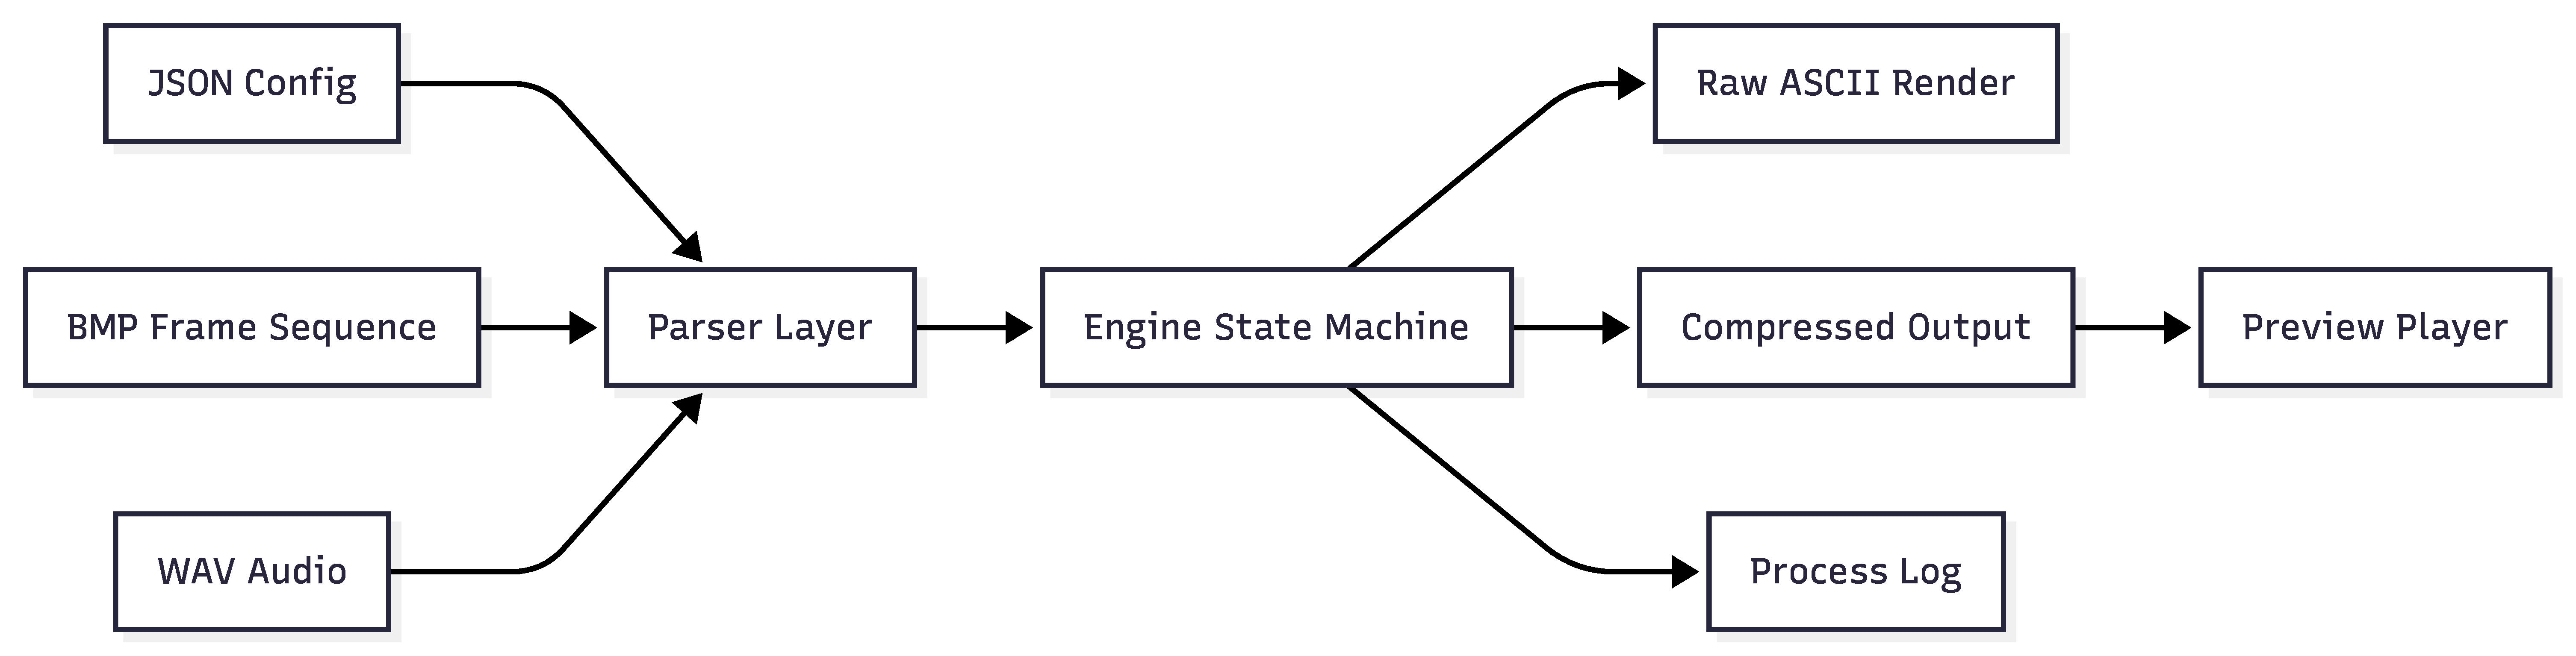
\includegraphics[width=0.75\textwidth]{figures/fig1.pdf}
    % flowchart LR
    % A[JSON Config] --> D[Parser Layer]
    % B[BMP Frame Sequence] --> D
    % C[WAV Audio] --> D
    % D --> E[Engine State Machine]
    % E --> F[Raw ASCII Render]
    % E --> G[Compressed Output]
    % E --> H[Process Log]
    % G --> I[Preview Player]
    \caption{High-level project pipeline used as a reading guide for the report.}
    \label{fig:system_overview_placeholder}
\end{figure}

\subsection{Reader Guide}
The rest of this report is organized as follows. Section 2 explains the architecture and data flow in detail, including module hierarchy and state-machine orchestration. Section 3 maps the implementation directly to the project constraints and grading criteria. Section 4 describes the development process for a two-member team and the integration strategy across subsystems. Section 5 discusses technical challenges and trade-offs encountered during implementation. Section 6 concludes with outcomes, lessons learned, and future improvements.

